
% \documentclass[11pt]{article}
% \documentclass[twocolumn]{article}

\documentclass{article}
\usepackage[margin=0.8in]{geometry}
\usepackage{multicol}


\usepackage{amsmath, amssymb, amsthm}
\usepackage{hyperref}
\usepackage{mathtools}
\usepackage{enumitem}
\usepackage{hyperref}
\hypersetup{
    colorlinks=false, % Set to true if you want colored text
    hidelinks         % This removes the red boxes completely
}


\title{Measuring Learning Efficiency via a Practical Information-Theoretic Approximation}
\author{Subhadeep Roy}
\date{2026/05/17}


\begin{document}
\maketitle

\begin{center}
\fbox{
\begin{minipage}{0.94\textwidth}
%\vspace{0.1cm}
{\Large \textbf{Reader's Guide (for quick review)}}
% \vspace{0.1cm}
\begin{itemize}
    \item See Section \ref{subsection:result1} for experimental results.
    \item Key finding: Models with similar accuracy can have large differences in information extraction.
    \item This helps distinguish model failure from intrinsic data uncertainty.
\end{itemize}

% \vspace{0.1cm}

\end{minipage}
}
\end{center}
\tableofcontents

\section{Objective}
The objective of this note is to develop a practical method for measuring the learning efficiency of predictive models 
relative to the intrinsic structure present in a dataset. 
In many machine learning settings, model performance is evaluated solely by accuracy or loss metrics, 
which makes it difficult to distinguish whether poor performance arises from model limitations or 
from the inherent unpredictability of the target variable given the available inputs. 
Information theory provides a principled way to characterize this distinction through the mutual information 
$I(X ; Y)$ which quantifies the amount of information the input variables $X$ contain about the 
target $Y$. 
However, direct estimation of mutual information in high-dimensional settings is typically intractable. 
This work proposes a practical approximation that uses negative log-likelihood (NLL) under a strong and 
well-calibrated reference model as a proxy for the conditional entropy 
$H(Y | X)$. This enables us to estimate a reasonable lower bound on the 
intrinsic learnability of a dataset, and a corresponding notion of model learning efficiency as the fraction of available information that a given model successfully extracts from that data.
\subsection{Scope and ongoing work}
The present formulation focuses on static datasets where samples are assumed 
to be independently drawn from a fixed distribution. This setting allows a 
clean estimation of intrinsic learnability via conditional entropy. 
Extending this framework to time-varying data where observations 
arrive sequentially and may exhibit temporal dependence is an active direction of ongoing work. 
In such settings, learnability becomes a property of the underlying stochastic process rather than a 
fixed dataset, requiring a causal formulation based on entropy-rates and history-dependent predictions.

% ===============================
% Prior Art Section
% ===============================
\section{Prior Art}

Our formulation builds on classical information theory, where mutual information $I(X;Y)=H(Y)-H(Y|X)$ 
characterizes the maximum information about labels that can, in principle, be extracted from inputs \cite{cover_thomas}. 
Log-loss provides a strictly proper scoring rule for probabilistic prediction \cite{gneiting_scoring}, 
and modern work on calibration evaluates the alignment between predicted probabilities and empirical outcomes \cite{guo_calibration}.

Recent work on scaling laws studies how predictive performance varies with model size, data volume, 
and compute \cite{kaplan2020scaling, hoffmann2022chinchilla}. 
These approaches identify regimes of diminishing returns and characterize compute-optimal model 
sizes for a given dataset. Related work also introduces data quality and redundancy as factors that influence effective scaling behavior \cite{quality_scaling}.

Complementary perspectives examine tradeoffs between compression and prediction at the representation level \cite{tishby_ib, grunwald_mdl}, 
as well as systems-level efficiency, where architectural and algorithmic optimizations reduce memory and compute requirements during inference \cite{llm_flash}.

Existing work does not explicitly separate the intrinsic information available in a dataset from the information actually extracted by a model. 
This distinction is central to our framework, which focuses on quantifying extraction efficiency relative to the dataset’s inherent predictability, 
rather than optimizing performance under compute or data constraints.

In practice, when intrinsic limits are unknown, strong models or ensembles are commonly used as empirical reference points. 
For example, teacher–student distillation frameworks use high-capacity models to define target behavior \cite{hinton2015distilling}, 
and scaling-law analyses evaluate performance across model families \cite{kaplan2020scaling} rather than against a theoretical bound, 
which is often computationally intractable.



\section{Limitations of Standard Model Evaluation}

Modern machine learning evaluation 
typically measures model performance using metrics such as accuracy, cross-entropy loss, 
or F1 score on a held-out dataset. 
While these metrics quantify predictive performance, they do not distinguish between two 
fundamentally different causes of error: model inefficiency and intrinsic unpredictability of the data. 
A model may perform poorly either because it fails to capture structure that exists in the data, 
or because the input variables simply do not contain sufficient information to reliably predict the target variable. 
In practice, these two scenarios are indistinguishable when evaluation relies solely on predictive accuracy.

This ambiguity becomes particularly problematic when evaluating new architectures, 
algorithms, or benchmarks. 
A low-performing model might suggest architectural deficiencies, 
but it could equally indicate that the dataset itself contains high levels of noise or irreducible uncertainty. 
Conversely, high performance may simply reflect a dataset with low intrinsic entropy rather than a particularly capable model.

Information theory provides a natural way to formalize this distinction. The mutual information $I(X ; Y)$  measures how much information the input variables 
$X$ contain about the target 
$Y$ and therefore represents the maximum predictive information 
that any model could extract from the data. While theoretical limits of this kind are well 
understood in principle, they are rarely estimated in practice for real-world datasets. 

As a result, models are typically evaluated only by their observed performance rather than by how close that performance is to the information limit imposed by the dataset.

To make this ambiguity precise, consider the commonly used F1 score 
for binary classification. 
Let $\hat{Y} = f(X) \in \{0,1\}$ denote the predicted label. 
The F1 score is defined as the harmonic mean of precision and recall and depends only on the joint distribution $p(\hat{Y}, Y)$. 
As such, it evaluates predictive performance purely in terms of agreement 
between predicted and true labels, without reference to the input variables $X$. This leads to a fundamental limitation: 
the F1 score does not capture how much information about $Y$ is actually available in $X$. Consequently, 
two qualitatively different scenarios may yield identical F1 scores. In the first, 
the dataset may be intrinsically unpredictable, with $H(Y \mid X) \approx H(Y)$ and $I(X; Y) \approx 0$, so that even the Bayes-optimal classifier performs poorly.
 In the second, the dataset may contain substantial predictive structure, with $H(Y \mid X) \ll H(Y)$, but the model fails to 
 approximate the true conditional distribution. In both cases, the observed F1 score may be low, yet the underlying causes are fundamentally different. 
 Moreover, the F1 score lacks a notion of a dataset-dependent performance ceiling: the maximum achievable F1 depends on the unknown 
 distribution $p(Y \mid X)$ and is therefore not accessible in practice. As a result, standard evaluation metrics measure what a model 
 achieves, but not how close it operates to the information-theoretic limits imposed by the dataset.

\section{Dataset Learnability}

A central question in predictive modeling is how much 
information about the target variable is actually present in the input data. Intuitively, 
if the inputs contain little information about the target, then even an ideal model cannot 
achieve high predictive accuracy. 
Conversely, if the inputs contain substantial information about the target, 
then poor model performance indicates that the model has failed to 
extract structure that exists in the data. We refer to the intrinsic predictability of a dataset as its \textit{learnability}.

Let the dataset consist of input variables $X$ and target variable $Y$ 
jointly distributed according to an unknown distribution $p(X,Y)$. 
This formulation assumes a static dataset setting where samples are independently drawn from this distribution.
The marginal distributions are denoted by $p(X)$ and $p(Y)$, and the conditional distribution of the target given the input is $p(Y|X)$.
The entropy of the target variable is defined as

\[
H(Y) = - \sum_{y} p(y)\log p(y)
\]
which measures the total uncertainty in the labels before observing the input.
The conditional entropy of the target given the input is

\[
H(Y|X) = - \mathbb{E}_{p(X,Y)}[\log p(Y|X)]
\]
which measures the residual uncertainty in the target after observing the input.
The reduction in uncertainty obtained by observing the input is quantified by the mutual information

\[
I(X;Y) = H(Y) - H(Y|X)
\]
which measures how much information the input variables contain about the target.
We define the \textit{learnability} of the dataset as the fraction of label uncertainty that can, in principle, be resolved using the input:

\[
L(X,Y) = \frac{I(X;Y)}{H(Y)} = 1 - \frac{H(Y|X)}{H(Y)}
\]

This normalization ensures that learnability lies in the interval $[0,1]$. When $L(X,Y)=0$, the inputs contain no information about the target, and prediction is fundamentally impossible. When $L(X,Y)=1$, the target is fully determined by the inputs.

In practice, computing $L(X,Y)$ requires estimating the conditional entropy $H(Y|X)$, which depends on the true conditional distribution $p(Y|X)$. For realistic datasets this distribution is unknown and generally intractable to estimate directly.

To obtain a practical approximation, we instead train a high-capacity \textit{golden model} $G$ whose purpose is to approximate the true conditional distribution. Let the predictive distribution of this model be denoted by $q_G(Y|X)$, where

\[
q_G(Y|X) \approx p(Y|X)
\]

Under this approximation, the conditional entropy can be estimated using the negative log-likelihood of the golden model:

\[
H(Y|X) \approx - \mathbb{E}_{p(X,Y)}[\log q_G(Y|X)]
\]

This expectation can be estimated empirically on held-out data as follows.

\subsection{Estimating the Posterior Density of the Data Labels}
Let the dataset be
\[
\mathcal{D}=\{(x_i,y_i)\}_{i=1}^{n},
\qquad y_i \in \{1,\dots,K\}.
\]
The probabilistic predictor $G$ returns a categorical distribution over labels:
\[
G(x) \equiv q_G(\cdot \mid x)\in\Delta^{K-1}, \qquad
q_G(k\mid x)\ge 0,\quad \sum_{k=1}^K q_G(k\mid x)=1.
\]
(Throughout, logarithms are base-2 (units: \emph{bits}). Switching to natural logs yields units of \emph{nats}.)

\subsubsection{Empirical Label Entropy}
Let the empirical class probabilities be
\[
\hat p(k) \;=\; \frac{1}{n}\sum_{i=1}^{n}\mathbf{1}\{y_i=k\}.
\]
The empirical label entropy is
\[
\hat H(Y) \;=\; -\sum_{k=1}^{K}\hat p(k)\log_2 \hat p(k),
\]
with the convention $0\log 0 \equiv 0$.

\subsubsection{Empirical Negative Log-Likelihood - NLL}
For a single example $(x_i,y_i)$, the negative log-likelihood under model $G$ is
\[
\ell_i(G) \;=\; -\log_2 q_G(y_i\mid x_i).
\]
Here $q_G(y_i \mid x_i)$ denotes the probability assigned by the model $G$
to the true label $y_i$ given input $x_i$. In general this probability
is typically strictly less than 1 in stochastic or noisy settings (the probability mass function is smeared around the true label). 
The per-sample negative log-likelihood
$\ell_i(G)$ therefore measures the information (in bits) associated with
the event that the model assigns probability $q_G(y_i \mid x_i)$ to the
observed label.
The empirical NLL over a dataset $\mathcal{D}$ is the sample mean
\[
\widehat{\mathrm{NLL}}_G(\mathcal{D})
\;=\;
\frac{1}{n}\sum_{i=1}^{n} \ell_i(G)
\;=\;
-\frac{1}{n}\sum_{i=1}^{n}\log_2 q_G(y_i\mid x_i).
\]
$\widehat{\mathrm{NLL}}_G$ as estimated above can serve as an upper bound to the true conditional entropy as:
\[
\widehat{\mathrm{NLL}}_G \geq H(Y | X)
\]
Consequently, learnability, expressed as the normalized information contained in the dataset can be approximated by the 
golden model $G$ as :

\[
\boxed{
L_G(X,Y) \approx 1 - \frac{\widehat{\mathrm{NLL}}_G }{\hat H(Y) }
}
\]
Because the golden model only approximates the true posterior distribution, 
the resulting estimate constitutes a \textit{lower bound} on the true learnability ceiling. 
The gap between the estimated learnability and the true value depends on how well the golden model approximates $p(Y|X)$, 
and therefore on the representational capacity and training quality of $G$.

\textbf{Evaluation protocol.} To approximate generalization, $\widehat{\mathrm{NLL}}_G$ should be computed on held-out data (validation/test or out-of-fold predictions), not on the training set.


\section{Model Efficiency}
Noting, that the above framework solely captures the learnability of the dataset (with $G$ being an oracle estimator - used offline for evaluation), we now
discuss the canonical efficiency of a given model under test: $F$. We pass the model $F$ through the above framework to calculate the normalized mutual 
information between the true labels $Y$ and the labels $F(X)$ predicted by $F$ as:
\begin{equation}
I_n(F(X);Y) = 1 - \frac{H(Y\mid F(X))}{H(Y)}   \approx 1 - \frac{\widehat{\mathrm{NLL}}_F}{\hat H(Y)}
\end{equation}
and finally normalize it to calculate the efficiency factor as:

% \begin{equation}
% I(F(X);Y) = H(Y) - H(Y\mid f(X)) \approx \hat H(Y) - \widehat{\mathrm{NLL}}_F 
% \end{equation},


\begin{equation}
\boxed{
    \eta(f)\;\coloneqq\;\frac{I_n(F(X);Y)}{ L_G(X,Y)}.
}
\end{equation}



\section{Interpretation and Edge Cases}

This section discusses how the proposed quantities behave under several 
important regimes and clarifies how to interpret the resulting metrics.

\subsection{Interpretation of Learnability}

The dataset learnability $L_G(X,Y)$ measures the fraction of label entropy 
that can be explained by the input variables.

\begin{itemize}[leftmargin=2em]

\item \textbf{$L_G(X,Y)\approx 0$.}  
The inputs contain little information about the labels. 
Even an optimal model cannot achieve reliable prediction, and performance 
near random guessing is expected.

\item \textbf{$L_G(X,Y)\approx 1$.}  
The labels are almost fully determined by the inputs. 
High predictive accuracy should in principle be achievable.

\item \textbf{Intermediate values.}  
Most real datasets fall in this regime, where part of the label entropy 
is predictable and the rest represents irreducible uncertainty or noise.

\end{itemize}

\subsection{Interpretation of Model Efficiency}

The efficiency score

\[
\eta(f) = \frac{I_n(F(X);Y)}{L_G(X,Y)}
\]

measures the fraction of available information that the model $F$ extracts 
from the dataset.

\begin{itemize}[leftmargin=2em]

\item \textbf{$\eta(f)\approx 1$.}  
The model extracts nearly all of the information available in the dataset. 
Further architectural improvements are unlikely to produce large gains 
unless the dataset itself changes.

\item \textbf{$\eta(f)\ll 1$.}  
The dataset contains predictive structure that the model fails to capture. 
Model improvements may significantly increase performance.

\end{itemize}

\subsection{Noiseless Targets}

If the labels are deterministic functions of the inputs, then

\[
H(Y|X)=0.
\]

In this case the intrinsic learnability is

\[
L(X,Y)=1.
\]

If both the golden model $G$ and the evaluated model $F$ perfectly capture 
the mapping, their NLL approaches zero and the estimated mutual information 
approaches the label entropy:

\[
I(F(X);Y) \to H(Y).
\]

\subsection{Irreducible Label Noise}

When the target contains stochastic components, the conditional entropy

\[
H(Y|X) > 0
\]

even for the Bayes-optimal predictor. In this setting the negative 
log-likelihood cannot approach zero, and the achievable predictive 
performance is fundamentally limited by the noise level of the dataset.

\subsection{Random Labels}

If labels are statistically independent of the inputs, then

\[
I(X;Y)=0.
\]

Consequently the learnability approaches

\[
L(X,Y)\approx 0.
\]

In this regime any model, regardless of complexity, performs no better 
than random guessing. This case serves as a useful sanity check for the 
framework.

\subsection{Overconfident Models}

The NLL metric penalizes models that assign high confidence to incorrect 
predictions. An overconfident but inaccurate model may therefore achieve 
poor NLL even if its classification accuracy appears reasonable. 
This behavior is desirable because the proposed framework measures the 
information conveyed by the \textbf{ \textit{full predictive distribution rather than 
only the top predicted label}}.

\subsection{Probabilistic Predictions}

The framework requires models to produce probabilistic outputs 
$q_F(y|x)$. Hard-label predictions discard uncertainty information and 
prevent accurate estimation of conditional entropy. For deterministic 
classifiers, probability calibration techniques may be required before 
computing NLL-based quantities.

\subsection{Extension to Time-Varying Data (Work in Progress)}
In many real-world systems, data is generated sequentially and exhibits temporal dependence. 
Examples include sensor streams, financial time series, and interactive systems. 
In such settings, the assumption of independently sampled $(X,Y)$ pairs no longer holds, and the notion of learnability must be generalized.

A natural extension is to define learnability over sequences $(X_{1:T}, Y_{1:T})$
, where prediction at time $t$ depends on the history $X_{1:t}$. 
The corresponding intrinsic uncertainty is governed by conditional 
entropy rates rather than single-step conditional entropy. 
This leads to a time-indexed notion of learnability that varies along the trajectory and reflects the evolving predictability of the process.
Developing a practical approximation of this sequential learnability, analogous to the NLL-based estimator proposed here, remains an open direction for future work.


\section{Validation on Synthetic Dataset}
This section describes the validation plan for the learnability framework
and demonstrate that negative log-likelihood (NLL) can be used to:
\begin{itemize}
\item Estimate a lower bound on the dataset learnability (intrinsic predictability).
\item Separate model inefficiency from intrinsic dataset uncertainty.
\end{itemize}
We generate an ensemble of synthetic datasets with varying degrees of learnability
and evaluate the framework on the ensemble. Since the dataset is synthetic, we have
full knowledge of the true posterior density of labels which gives us the true
underlying learnability of the ensemble. We will then run a high-powered
oracle model ($G$) to estimate the learnability of the ensemble, which will serve as a 
tight lower bound on the true learnability. This lower bound from the
oracle model will then be used as a baseline for computing the efficiency of a library of 
models under test.

\subsection{Dataset Construction}\label{subsec:DatasetConstruction}
Let $X \in \mathbb{R}^d$ denote the feature vector. 
We partition the feature space into subsets with different distributions to induce heterogeneous learnability:

\begin{align*}
    X = [X^{(1)}, X^{(2)}], \quad 
    X^{(1)} \in \mathbb{R}^{d_1}, \; X^{(2)} \in \mathbb{R}^{d_2}, \; d_1 + d_2 = d
\end{align*}

The feature subsets are drawn as:
\begin{align*}
    X^{(1)} &\sim \mathcal{N}(0, I_{d_1}) \\
    X^{(2)} &\sim \mathcal{D} \quad \text{(non-Gaussian or structured distribution)}
\end{align*}

where $\mathcal{D}$ can be chosen to control feature informativeness (e.g., heavy-tailed, bounded, or low-variance distributions).

The latent score is defined as:
\begin{align*}
    t(X) = \beta\, w^\top X
\end{align*}
where $w$ is a binary vector used to mask out a randomly selected feature subset.
The conditional label distribution is:
\begin{align*}
    p(y=1 \mid X) = \sigma(t(X)) = \frac{1}{1 + e^{-t(X)}}
\end{align*}

The binary label is then sampled as:
\[
y \sim \mathrm{Bernoulli}(p(y=1\mid X)).
\]

\paragraph{Controlling Learnability}
The learnability of the dataset is governed by three factors:

\begin{itemize}
    \item \textbf{Signal strength} ($\beta$): controls the separation between classes. For example:
    \begin{itemize}
        \item High learnability: $\beta = 4.0$
        \item Medium learnability: $\beta = 1.5$
        \item Low learnability: $\beta = 0.5$
    \end{itemize}

    \item \textbf{Sparsity of the signal} ($d'$): number of active dimensions in $w$ (number of 1's entries in $w$).
    The remaining $(d - d')$ components are set to zero.
    \begin{itemize}
        \item High learnability:   $d' = d$ (all features contribute)
        \item Medium learnability: $d' = \frac{d}{2}$
        \item Low learnability:    $d' = 1$
    \end{itemize}

    \item \textbf{Feature distribution heterogeneity}: controls how informative different subsets of $X$ are.
    \begin{itemize}
        \item High learnability: informative features concentrated in $X^{(1)}$ (Gaussian, well-conditioned)
        \item Medium learnability: signal spread across both $X^{(1)}$ and $X^{(2)}$
        \item Low learnability: signal concentrated in weak or noisy subset $X^{(2)}$
    \end{itemize}
\end{itemize}

This construction allows independent control over signal strength, sparsity, and feature distribution, enabling a richer spectrum of learnability regimes beyond isotropic Gaussian settings.

% \subsection{Ground Truth Learnability}
% For the synthetic Bernoulli model the true learnability is known and can be computed as
% \begin{align*}
%     H(Y\mid X) &= \mathbb{E}_X\!\left[h_2\!\big(\sigma(t(X))\big)\right] \\
%                &= \mathbb{E}_X\!\left[\log_2\!\bigl(1+e^{-t(X)}\bigr) + \frac{e^{-t(X)}}{1+e^{-t(X)}}\frac{t(X)}{\ln 2}\right]
% \end{align*}
% where
% \begin{align*}
%     h_2(p) = -p\log_2 p - (1-p)\log_2(1-p)
% \end{align*}
% is the binary entropy function. The true learnability is then
% \begin{align*}
% L_{\mathrm{true}} = 1 - \frac{H(Y\mid X)}{H(Y)}.
% \end{align*}
% In this synthetic construction, due to symmetry of the Gaussian input and the logistic link function, the marginal label distribution satisfies
% $p(y=1)=0.5$, yielding the theoretical label entropy $H(Y)=1$ bit. However in practice, we used the estimate of $\hat{H}(Y)$, which 
% may deviate from the true entropy due to finite sampling.




\section{Experimental Results}\label{section:experimental_results}

\subsection{Controlled Learnability using Synthetic Dataset}
The dataset is generated as described in section \ref{subsec:DatasetConstruction} with the following parameters
to control the learnability:

\begin{itemize}
    \item Signal strength: $0.5 < \beta \leq 10$
    \item Sparsity: $\frac{d'}{d} \in $ [0.1,  0.5,  1.0]
\end{itemize}

\vspace{0.3em}
\noindent
\textbf{Models.} We train fixed-depth MLPs with width ranging from 32 to 1024, 
thereby scaling capacity while keeping architecture constant.

\vspace{0.5em}
\noindent
\textbf{Metrics.} For each model $f$:
\begin{itemize}
    \item NLL(f): $-\mathbb{E}_{p(X,y)}[\log f(Y|X)]$
    \item F1 score (standard accuracy proxy)
    \item Model score: $\hat{\L}(f) = 1 - \frac{\mathrm{NLL}(f)}{H(Y)}$
    \item Efficiency: $\eta(f) = \frac{\hat{\L}(f)}{\L_{\text{true}}}$
\end{itemize}

Efficiency measures the fraction of extractable information captured by the model.

\subsubsection{Result 1: Same Accuracy, Different Information Extraction}\label{subsection:result1}
\begin{figure}[t]
    \centering
    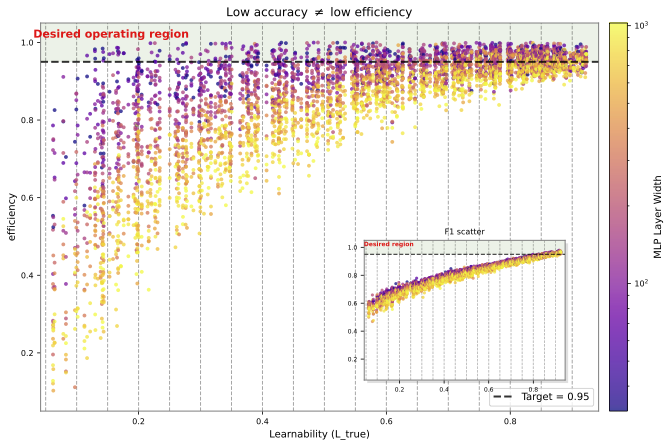
\includegraphics[width=0.9\linewidth]{figures/efficiency_scatter.png}
    \caption{Efficiency vs dataset learnability for different model sizes.}
    \label{figure:synthetic_eff_vs_learnability}
\end{figure}

Figure \ref{figure:synthetic_eff_vs_learnability} plots efficiency as a function of dataset learnability for models of different sizes.

\vspace{0.5em}
\noindent
\textbf{Key pattern:}
\begin{itemize}
    \item In high-learnability regimes, all models converge in both accuracy and efficiency 
    \item In low-learnability regimes, efficiency differs across model sizes, even when accuracy remains similar
\end{itemize}
Critically, the inset shows that:
\begin{quote}
    \begin{center}
        \emph{All models appear equivalent under F1 score.}
    \end{center}
\end{quote}
However,
\begin{itemize}
    \item Raw efficiency differs substantially across model sizes 
    \item Smaller models often achieve higher efficiency in low-learnability regimes
\end{itemize}
This indicates that two models with identical accuracy can still differ in their probabilistic alignment 
with the underlying data, particularly in low-signal regimes. We interpret this as metric decoupling where accuracy reflects correctness of discrete decisions while
efficiency reflects how much of the data's available signal is captured in the predictive distribution.

\subsubsection{Result 2: Capacity Scaling Beyond Data-Limited Regimes}

\begin{figure}[t]
    \centering
    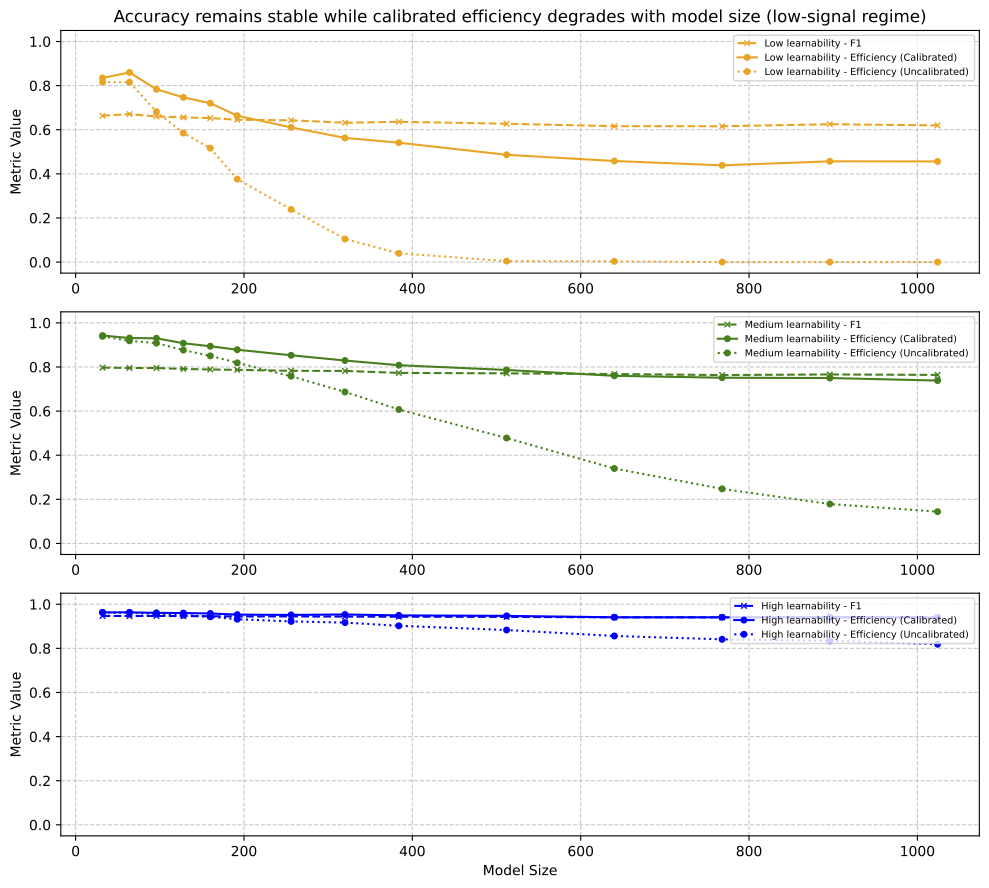
\includegraphics[width=0.9\linewidth]{figures/eff_vs_modelsize.png}
    \caption{Scaling model capacity beyond dataset learnability.}
    \label{figure:synthetic_eff_vs_modelsize}
\end{figure}

Figure \ref{figure:synthetic_eff_vs_modelsize} shows model scaling behavior as capacity increases for datasets with varying levels of intrinsic learnability.

\vspace{0.3em}
\noindent
\textbf{Observation:} Once model capacity exceeds the dataset’s effective learnability, 
further increases in capacity do not improve the amount of information extracted from the data, 
even though predictive accuracy remains largely unchanged.

More concretely:
\begin{itemize}
    \item F1 score remains nearly constant across model sizes.
    \item Raw NLL worsens with increasing capacity.
    \item After calibration, NLL improves substantially, but a residual gap remains.
    \item Efficiency decreases and approaches a lower plateau in low-learnability regimes.

\end{itemize}
This indicates that there exists a data-dependent capacity threshold beyond which, additional model capacity 
yields diminishing or negative returns in probabilistic fidelity,
does not improve predictive accuracy, and
reaches an efficiency-floor after optimal model calibration. We refer to this regime as \textbf{capacity-information saturation}:  

\begin{quote}
    \begin{center}
        \emph{Model capacity grows, but the amount of information extracted 
        from the data starts exhibiting diminishing, and sometimes negative, returns after calibration.}
    \end{center}
\end{quote}
Importantly, this behavior is not reflected in accuracy-based metrics, which remain stable across model sizes.

\subsection{Avazu Click Through Rate (CTR) Prediction - Work In Progress}
In this section we evaluate the framework on Avazu CTR prediction, 
a real-world tabular classification task with unknown intrinsic learnability. 
Since the true learnability is unavailable, we approximate a practical reference ceiling 
using the best calibrated held-out NLL among a family of strong tabular models, 
including gradient-boosted trees and TabTransformer. We then compare a small family of MLPs of 
increasing width against this empirical ceiling.



\section{Interpretation: Capacity--Information Saturation}

These results empirically separate two concepts that are often conflated:

\begin{itemize}
    \item \textbf{Learnability} ($L_{\text{true}}$): the intrinsic amount of predictable information present in the dataset
    \item \textbf{Efficiency} ($\eta$): how much of that available information a model actually extracts
\end{itemize}
When model capacity increases beyond the point at which the available signal is already well captured, further scaling does not increase the amount of extractable information. Instead, it produces diminishing returns in probabilistic fidelity and, in low-learnability regimes, may reduce efficiency even after calibration.

Formally,
\[
NLL(f) = H(Y|X) + \mathbb{E}_X D_{KL}\!\left(P^*(Y|X)\,\|\,f(Y|X)\right)
\]
This decomposition makes clear that held-out NLL differs from the intrinsic uncertainty $H(Y|X)$ by a mismatch term measuring how far the model's predictive distribution is from the true conditional distribution. In our experiments, calibration reduces a substantial part of this mismatch, but a residual gap remains in low-signal regimes as model size increases.

The resulting picture is not one of unbounded collapse, but of \textbf{capacity--information saturation}: beyond a dataset-dependent threshold, additional capacity does not yield additional extracted signal and may lead to lower efficiency.

\section{Implications}

Modern model selection is often dominated by accuracy-based metrics. These results show that:

\begin{itemize}
    \item Models can have similar predictive accuracy while differing substantially in information extraction efficiency.
    \item Increasing model capacity can yield diminishing or negative returns in probabilistic fidelity without materially improving accuracy.
    \item This effect is strongest in low-learnability regimes, where the data itself limits the amount of extractable signal.
\end{itemize}
The learnability--efficiency framework therefore provides a way to:
\begin{itemize}
    \item quantify the intrinsic predictability of synthetic datasets, and approximate practical reference ceilings when true limits are unknown.
    \item identify regimes in which calibration improves reliability but does not fully close the gap between model predictions and available signal.
    \item compare models based not only on decision correctness, but on how much information they extract from the data relative to what the data can support.
\end{itemize}
In this sense, the framework is not primarily a claim about model failure, but a tool for identifying when additional capacity is no longer justified by the information content of the dataset.




% ===============================
% References
% ===============================
\section{References}
\bibliographystyle{plain}
\bibliography{references}

\end{document}

















% \section{Learnability-Aware Decision Making}

% The framework developed thus far focuses on characterizing the intrinsic predictability of a dataset and the efficiency with which a model extracts that predictive information. However, in most practical settings, predictive models are not endpoints; rather, they serve as inputs to downstream decision-making systems.

% We now connect the notions of learnability and efficiency to a classical decision-theoretic framework.

% \subsection{Decision-Theoretic Setup}

% Let $\mathcal{A}$ denote a set of possible actions, and let
% \[
% u : \mathcal{A} \times \mathcal{Y} \rightarrow \mathbb{R}
% \]
% be a utility function assigning a real-valued reward to each action-outcome pair.

% Given an input $x$ and a predictive model $F$ with conditional distribution $q_F(y|x)$, the optimal action under model $F$ is given by:
% \[
% a_F(x) = \arg\max_{a \in \mathcal{A}} \mathbb{E}_{q_F(y|x)}[u(a,y)].
% \]

% The resulting expected utility achieved by model $F$ is:
% \[
% U(F) = \mathbb{E}_{p(x,y)} \left[ u(a_F(x), y) \right].
% \]

% This formulation makes explicit the separation between:
% \begin{itemize}
%     \item \textbf{Inference}: estimation of $q_F(y|x)$
%     \item \textbf{Decision}: maximization of expected utility
% \end{itemize}

% \subsection{Role of Learnability and Efficiency}

% The expected utility $U(F)$ depends critically on the quality of the predictive distribution $q_F(y|x)$. However, standard evaluation metrics such as accuracy or NLL do not distinguish between errors arising from intrinsic uncertainty in the data and those arising from model inefficiency.

% The learnability-efficiency decomposition introduced earlier provides a principled way to make this distinction:
% \begin{itemize}
%     \item Learnability $L_G(X,Y)$ quantifies the total predictive information available in the dataset
%     \item Efficiency $\eta(f)$ quantifies the fraction of that information captured by the model
% \end{itemize}

% Thus, efficiency can be interpreted as a measure of how much \emph{usable signal} a model makes available for downstream decision-making.

% \subsection{Learnability-Aware Model Selection}

% Consider two models $F_1$ and $F_2$ with similar predictive performance (e.g., similar NLL). Without additional context, selecting between them is ambiguous. However, if $\eta(f_1) > \eta(f_2)$, then $F_1$ extracts a larger fraction of the available information in the dataset and therefore provides a more faithful approximation to the true conditional distribution.

% In decision-theoretic terms, this implies that the action $a_{F_1}(x)$ is computed using a more informative posterior than $a_{F_2}(x)$, and is therefore expected to yield higher utility under a wide class of utility functions.

% Importantly, this reasoning is independent of the specific form of the utility function $u(a,y)$. The efficiency metric does not prescribe a particular decision rule, but rather quantifies the quality of the probabilistic input to any such rule.

% \subsection{Efficiency as a Model Reliability Signal}

% An alternative interpretation is to view efficiency as a measure of model reliability. Given a collection of models $\{F_j\}$, one may form an aggregated predictive distribution:
% \[
% \tilde{q}(y|x) = \frac{1}{Z} \sum_j \eta(f_j)\, q_{F_j}(y|x),
% \]
% where $Z$ is a normalization constant.

% This can be interpreted as an efficiency-weighted model averaging scheme, where models that extract more information from the dataset contribute more strongly to the final predictive distribution. The resulting distribution $\tilde{q}(y|x)$ can then be used within the same decision rule:
% \[
% a(x) = \arg\max_{a \in \mathcal{A}} \mathbb{E}_{\tilde{q}(y|x)}[u(a,y)].
% \]

% \subsection{Implications}

% The key implication of this framework is that model evaluation should not be performed solely in terms of predictive performance, but rather in terms of how close a model operates to the intrinsic information limit of the dataset.

% By explicitly estimating this limit and normalizing model performance against it, the proposed framework provides:
% \begin{itemize}
%     \item A principled method for distinguishing model inefficiency from intrinsic uncertainty
%     \item A model-agnostic signal for selecting models under arbitrary utility functions
%     \item A foundation for incorporating model efficiency directly into downstream decision-making
% \end{itemize}

% In this sense, learnability and efficiency form an intermediate layer between statistical inference and decision theory, enabling more informed and robust decision-making in practical systems.

